\section{Proving sorting network correctness}

\renewcommand{\CURPATH}{proofs/sorting_network}

Sorting networks are highly popular in electronics, GPGPU and even in SAT encodings:
\url{https://en.wikipedia.org/wiki/Sorting_network}.

Especially bitonic sorters, which are also sorting networks:
\url{https://en.wikipedia.org/wiki/Bitonic_sorter}.

Its popularity is probably related to the fact they can be parallelized easily.

They are relatively easy to construct, but, finding a smallest possible is a challenge.

There is a smallest network (only 25 comparators) for 9-channel sorting network:

\begin{figure}[H]
\centering
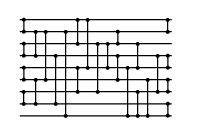
\includegraphics[scale=0.75]{\CURPATH/network9.png}
\caption{Smallest possible}
\end{figure}

This is combinational circuit, each connection is a comparator+swapper, it swaps if one of input values is bigger and passes output to the next level.

I copypasted it from \href{https://arxiv.org/pdf/1405.5754.pdf}{the article}:
Michael Codish, Lu ́ıs Cruz-Filipe, Michael Frank, and Peter Schneider-Kamp --
``Twenty-Five Comparators is Optimal when Sorting Nine Inputs (and Twenty-Nine for Ten)''.

Another article about it: \href{http://larc.unt.edu/ian/pubs/9-input.pdf}{Ian Parberry -- A Computer Assisted Optimal Depth Lower Bound for Nine-Input Sorting Networks}.

I don't know (yet) how they proved it, but it's interesting, that it's extremely easy to prove its correctness using Z3 SMT solver.
We just construct network out of comparators/swappers and asking Z3 to find counterexample, for which the output of the network will not be sorted.
And it can't, meaning, output's state is always sorted, no matter what values are plugged into inputs.

\lstinputlisting[style=custompy]{\CURPATH/test9.py}

( The full source code: \url{https://github.com/DennisYurichev/SAT_SMT_by_example/blob/master/proofs/sorting_network/test9.py}. )

There is also smaller 4-channel network I copypasted from Wikipedia:

\begin{lstlisting}
...

l=line(l, " + +")
l=line(l, "+ + ")
l=line(l, "++++")
l=line(l, " ++ ")

...
\end{lstlisting}

( The full source code: \url{https://github.com/DennisYurichev/SAT_SMT_by_example/blob/master/proofs/sorting_network/test4.py}. )

It also proved to be correct, but it's interesting, what Z3Py expression we've got at each of 4 outputs:

\begin{lstlisting}
If(If(a < c, a, c) < If(b < d, b, d),
   If(a < c, a, c),
   If(b < d, b, d))

If(If(If(a < c, a, c) > If(b < d, b, d),
      If(a < c, a, c),
      If(b < d, b, d)) <
   If(If(a > c, a, c) < If(b > d, b, d),
      If(a > c, a, c),
      If(b > d, b, d)),
   If(If(a < c, a, c) > If(b < d, b, d),
      If(a < c, a, c),
      If(b < d, b, d)),
   If(If(a > c, a, c) < If(b > d, b, d),
      If(a > c, a, c),
      If(b > d, b, d)))

If(If(If(a < c, a, c) > If(b < d, b, d),
      If(a < c, a, c),
      If(b < d, b, d)) >
   If(If(a > c, a, c) < If(b > d, b, d),
      If(a > c, a, c),
      If(b > d, b, d)),
   If(If(a < c, a, c) > If(b < d, b, d),
      If(a < c, a, c),
      If(b < d, b, d)),
   If(If(a > c, a, c) < If(b > d, b, d),
      If(a > c, a, c),
      If(b > d, b, d)))

If(If(a > c, a, c) > If(b > d, b, d),
   If(a > c, a, c),
   If(b > d, b, d))
\end{lstlisting}

The first and the last are shorter than the 2nd and the 3rd, they are just
$min(min(min(a,b),c),d)$ and 
$max(max(max(a,b),c),d)$.

